% =========================================================
% prezentace.tex -- Taylorovy rady: Beamer prezentace
% Seminar IVT, 3. rocnik gymnazia
%
% Kompilace: XeLaTeX
%   latexmk -pdf -cd prezentace/prezentace.tex
% =========================================================

\documentclass[12pt]{beamer}

% --- Téma ---
\usetheme{Madrid}
\usecolortheme{default}

% --- Okraje snímků ---
\setbeamersize{text margin left=6mm, text margin right=6mm}

% --- Čeština ---
\usepackage{polyglossia}
\setmainlanguage{czech}
\usepackage{fontspec}

% --- Matematika ---
\usepackage{amsmath}

% --- Čísla s desetinnou čárkou ---
\usepackage{siunitx}
\sisetup{
    output-decimal-marker = {,},
    group-separator       = {\,},
}

% --- Grafika ---
\usepackage{graphicx}

% --- Tabulky ---
\usepackage{booktabs}

% --- TikZ ---
\usepackage{tikz}

% --- Zdrojový kód ---
\usepackage{xcolor}
\usepackage{listings}

\definecolor{codebg}{RGB}{245,245,245}
\definecolor{codegreen}{RGB}{0,120,0}
\definecolor{codepurple}{RGB}{120,0,140}
\definecolor{codeblue}{RGB}{0,0,180}

\lstdefinestyle{pyslide}{
    language=Python,
    backgroundcolor=\color{codebg},
    basicstyle=\ttfamily\footnotesize,
    keywordstyle=\color{codeblue}\bfseries,
    commentstyle=\color{codegreen}\itshape,
    stringstyle=\color{codepurple},
    breaklines=true,
    showstringspaces=false,
    frame=single,
    framerule=0.4pt,
    tabsize=4,
    numbers=left,
    numberstyle=\tiny\color{gray},
    numbersep=6pt,
}
\lstset{style=pyslide}

% --- Uvozovky ---
\usepackage{csquotes}
\newcommand{\uv}[1]{\enquote{#1}}

% --- Bibliografie ---
\usepackage[backend=biber, style=iso-numeric, sorting=none]{biblatex}
\addbibresource{../literatura.bib}

% =========================================================
% Titulní informace
% =========================================================
\title{Taylorovy řady}
\subtitle{Jak kalkulačka počítá sinus?}
\author{Seminář IVT}
\institute{3.~ročník gymnázia}
\date{2025}

% =========================================================
\begin{document}
% =========================================================

% ----------------------------------------------------------
% SNÍMEK 1: Titulní strana
% ----------------------------------------------------------
\begin{frame}
    \titlepage
\end{frame}

% ----------------------------------------------------------
% SNÍMEK 2: Obsah
% ----------------------------------------------------------
\begin{frame}{Obsah}
    \tableofcontents
\end{frame}

% ==========================================================
\section{Motivace}
% ==========================================================

% ----------------------------------------------------------
% SNÍMEK 3: Co dělá kalkulačka?
% ----------------------------------------------------------
\begin{frame}{Co dělá kalkulačka, když stisknete sin?}

    \begin{columns}
        \column{0.55\textwidth}
        \begin{itemize}
            \item Zadáme $30^\circ$, dostaneme $0{,}5$.
            \pause
            \item Jak to vypočítá? Neexistuje \uv{jednoduchý} vzorec.
            \pause
            \item Kalkulačka používá \textbf{aproximační algoritmus}.
        \end{itemize}

        \bigskip
        \begin{block}{Dnešní cíl}
            Naučit se \textbf{Taylorovu řadu} ---
            základ pro pochopení aproximací.
        \end{block}

        \column{0.4\textwidth}
        \centering
        \begin{block}{Používané metody}
            \begin{itemize}
                \item Maclaurin / Taylor
                \item Čebyšev
                \item CORDIC
                \item Tabulky
            \end{itemize}
        \end{block}
    \end{columns}

\end{frame}

% ----------------------------------------------------------
% SNÍMEK 4: Přehled metod
% ----------------------------------------------------------
\begin{frame}{Metody používané v~praxi}

    \begin{block}{Maclaurinovy řady (Taylor v~bodě 0)}
        Nekonečný polynom. Intuitivní, výchozí bod.
        Pro velká $x$ konverguje pomalu.
    \end{block}

    \pause

    \begin{exampleblock}{Čebyševovy polynomy}
        Minimalizují maximální chybu na daném intervalu.
        Přesnější při stejném počtu koeficientů.
    \end{exampleblock}

    \pause

    \begin{block}{CORDIC~\cite{volder1959}}
        Jen bitové posuvy a sčítání. Žádné násobení.
        Vhodný pro jednoduché čipky (digitální hodinky, GPS).
    \end{block}

    \pause

    \begin{alertblock}{My studujeme Taylor}
        Konverguje pomaleji, ale je \textbf{intuitivní}
        a je \textbf{výchozím bodem} pro všechny ostatní metody.
    \end{alertblock}

\end{frame}

% ==========================================================
\section{Taylorova řada}
% ==========================================================

% ----------------------------------------------------------
% SNÍMEK 5: Co je Taylorova řada
% ----------------------------------------------------------
\begin{frame}{Taylorova řada --- idea}

    \begin{block}{Klíč}
        Každá hladká funkce lze \textbf{lokálně přiblížit polynomem}.
        Čím více členů, tím přesnější aproximace.
    \end{block}

    \pause
    \bigskip

    \textbf{Maclaurinova řada} ($a = 0$):
    \[
        f(x) = f(0) + f'(0)\cdot x
               + \frac{f''(0)}{2!} x^2
               + \frac{f'''(0)}{3!} x^3 + \cdots
    \]

    \pause
    \begin{exampleblock}{Intuice bez derivací}
        Člen $x$ = tečna ke křivce v~$x_0 = 0$.
        Člen $x^3$ = opravuje zakřivení.
        Každý další člen opravuje chybu předchozího.
    \end{exampleblock}

\end{frame}

% ==========================================================
\section{Sinus a kosinus}
% ==========================================================

% ----------------------------------------------------------
% SNÍMEK 6: sin(x) -- vzorec + vizualizace
% ----------------------------------------------------------
\begin{frame}{$\sin(x)$ --- Maclaurinova řada}

    \[
        \sin(x)
        = x - \frac{x^3}{3!} + \frac{x^5}{5!} - \frac{x^7}{7!} + \cdots
    \]

    \medskip
    \textbf{Pozor:} $x$ musí být v~\textbf{radiánech}.
    ($30^\circ = \pi/6 \approx \num{0.5236}$~rad)

    \pause
    \medskip

    \begin{center}
    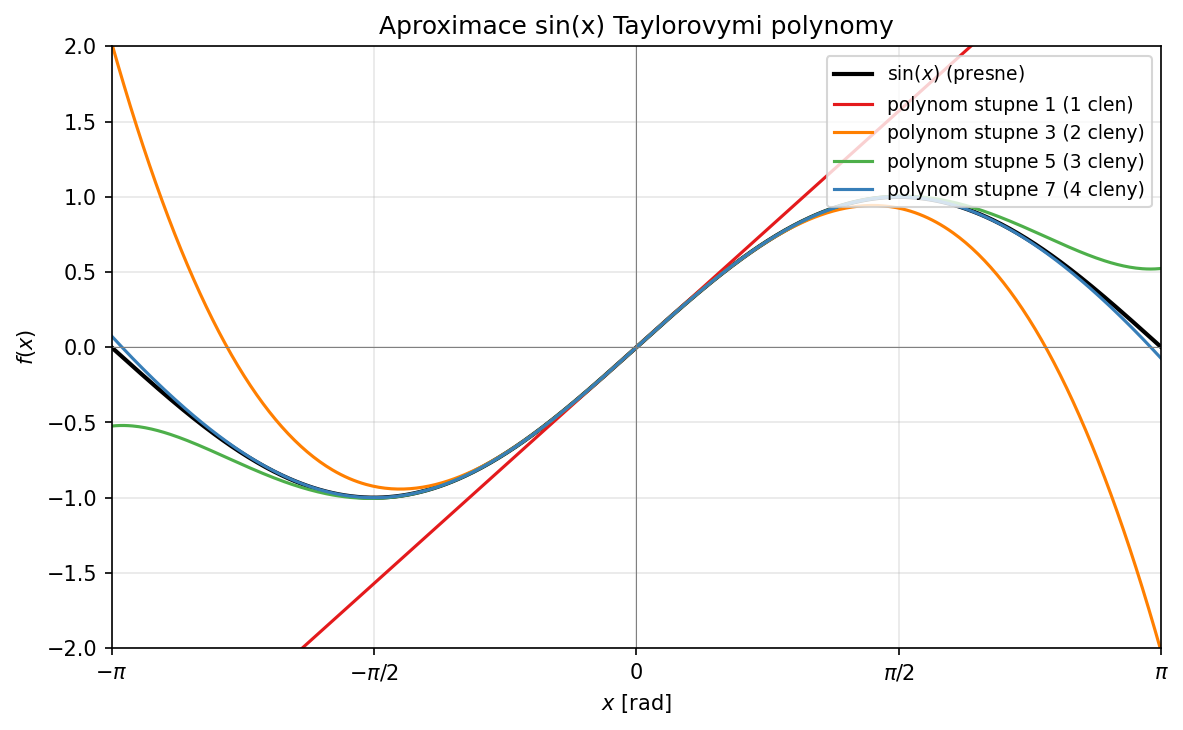
\includegraphics[width=0.75\textwidth]{../python/output/sin_aproximace.png}
    \end{center}

\end{frame}

% ----------------------------------------------------------
% SNÍMEK 7: cos(x) -- vzorec
% ----------------------------------------------------------
\begin{frame}{$\cos(x)$ --- Maclaurinova řada}

    \[
        \cos(x)
        = 1 - \frac{x^2}{2!} + \frac{x^4}{4!} - \frac{x^6}{6!} + \cdots
    \]

    \pause
    \bigskip

    \begin{columns}
        \column{0.48\textwidth}
        \begin{block}{Sinus --- liché mocniny}
            $x,\; x^3,\; x^5,\; x^7, \ldots$\\
            Začíná členem $x$.
        \end{block}

        \column{0.48\textwidth}
        \begin{block}{Kosinus --- sudé mocniny}
            $1,\; x^2,\; x^4,\; x^6, \ldots$\\
            Začíná členem $1$.
        \end{block}
    \end{columns}

    \pause
    \bigskip

    \begin{exampleblock}{Konvergence}
    Pro $x \in [-\pi, \pi]$ stačí \textbf{10 členů}
    pro přesnost lepší než $10^{-12}$.
    \end{exampleblock}

\end{frame}

% ==========================================================
\section{Odmocnina}
% ==========================================================

% ----------------------------------------------------------
% SNÍMEK 8: Newtonova iterace
% ----------------------------------------------------------
\begin{frame}{Odmocnina --- Newtonova iterace}

    \begin{block}{Myšlenka: lepší a lepší odhad}
        \begin{enumerate}
            \item<1-> Počáteční odhad: $x_0 = a$
            \item<2-> Každý krok:
                \[
                    x_{n+1} = \frac{x_n + \dfrac{a}{x_n}}{2}
                \]
            \item<3-> Jen $+$, $\times$ a $/$ --- žádné mocniny.
        \end{enumerate}
    \end{block}

    \onslide<4->{
    \begin{alertblock}{Kvadratická konvergence}
        Počet správných číslic se přibližně \textbf{zdvojuje}
        při každé iteraci!
    \end{alertblock}
    }

\end{frame}

% ----------------------------------------------------------
% SNÍMEK 9: Babylonský příběh -- YBC 7289
% ----------------------------------------------------------
\begin{frame}{3700 let stará metoda --- tabulka YBC~7289}

    \begin{columns}
        \column{0.54\textwidth}
        \begin{itemize}
            \item Kolem roku \textbf{1700 př.~n.~l.}
            \pause
            \item Babylonský písař zapsal $\sqrt{2}$
                  na hliněnou tabulku.
            \item Přesnost: \textbf{6 platných číslic}.
            \pause
            \item Sexagesimální (základ 60) zápis:\\
                  $1;\; 24,\; 51,\; 10$\\
                  $= 1 + \tfrac{24}{60} + \tfrac{51}{3600}
                    + \tfrac{10}{216000}$\\
                  $\approx \num{1.41421}$
        \end{itemize}

        \column{0.43\textwidth}
        \begin{alertblock}{Stejný algoritmus}
            Přesně ta iterace,\\
            kterou jsme právě ukázali!
            \[
                x_{n+1} = \frac{x_n + a/x_n}{2}
            \]
            Nezávisle znovuobjevena:\\
            Heron (1.~stol.\ n.~l.),\\
            Newton (17.~stol.)
        \end{alertblock}
    \end{columns}

\end{frame}

% ----------------------------------------------------------
% SNÍMEK 10: Geometrie Newtonovy iterace -- TikZ
% ----------------------------------------------------------
\begin{frame}{Geometrie: tečna k~parabolě}

    \begin{columns}
        \column{0.42\textwidth}
        \begin{block}{Postup pro $\sqrt{a}$}
            \begin{enumerate}
                \item Bod $(x_n,\, x_n^2)$ na $y=x^2$
                \item Tečna protíná $y = a$
                \item Průsečík = $x_{n+1}$
                \item Opakovat
            \end{enumerate}
        \end{block}
        \medskip
        \small
        Tečna v~$(x_n, x_n^2)$, sklon $2x_n$:\\
        \[
            x_{n+1} = \frac{x_n + a/x_n}{2}
        \]

        \column{0.55\textwidth}
        \centering
        \begin{tikzpicture}[x=2.5cm, y=0.65cm, >=latex, font=\scriptsize]
          \draw[->] (1.15,0) -- (2.2,0) node[right] {$x$};
          \draw[->] (1.15,0) -- (1.15,4.6) node[above] {$y$};
          \foreach \yy in {1,2,3,4}
            \draw (1.15,\yy) -- (1.12,\yy) node[left] {\yy};
          \draw[domain=1.2:2.07, smooth, very thick, blue!70!black, samples=50]
            plot (\x, {\x*\x});
          \node[right=2pt, blue!70!black] at (2.07,{2.07*2.07}) {$y=x^2$};
          \draw[gray!70, dashed, thick] (1.15,2) -- (2.12,2)
            node[right, gray!80!black] {$y=a$};
          % Krok 1
          \draw[red!25, dashed] (2,0) -- (2,4);
          \node[below, red!80!black] at (2,0) {$x_0$};
          \filldraw[red] (2,4) circle (2pt);
          \draw[red, very thick] (2,4) -- (1.5,2);
          % Krok 2
          \draw[orange!35, dashed] (1.5,0) -- (1.5,2.25);
          \node[below, orange!80!black] at (1.5,0) {$x_1$};
          \filldraw[orange!80!black] (1.5,2.25) circle (2pt);
          \draw[orange!80!black, very thick] (1.5,2.25) -- (1.4167,2);
          % x_2
          \filldraw[green!60!black] (1.4167,2) circle (2pt);
          \node[above left=-1pt, green!60!black] at (1.4167,2)
            {$x_2\!\approx\!\sqrt{2}$};
        \end{tikzpicture}
    \end{columns}

\end{frame}

% ----------------------------------------------------------
% SNÍMEK 11: sqrt(2) -- průchod iterací
% ----------------------------------------------------------
\begin{frame}{$\sqrt{2}$ --- průchod iterací}

    \begin{center}
    \begin{tabular}{@{}rll@{}}
    \toprule
    Iterace & $x_n$            & Chyba         \\ \midrule
    0       & $2{,}000000$     & $\num{5.9e-1}$ \\
    1       & $1{,}500000$     & $\num{8.6e-2}$ \\
    2       & $1{,}416667$     & $\num{2.5e-3}$ \\
    3       & $1{,}414216$     & $\num{2.1e-6}$ \\
    4       & $1{,}414214$     & $\num{1.6e-12}$ \\
    5       & $1{,}414214$     & $< 10^{-15}$ \\
    \bottomrule
    \end{tabular}
    \end{center}

    \medskip
    \centering
    \small Správná hodnota: $\sqrt{2} = \num{1.41421356}\ldots$

\end{frame}

% ==========================================================
\section{Python}
% ==========================================================

% ----------------------------------------------------------
% SNÍMEK 10: sin_taylor -- kód
% ----------------------------------------------------------
\begin{frame}[fragile]{Python: \texttt{sin\_taylor}}

\begin{lstlisting}
def faktorial(n):
    vysledek = 1
    for i in range(2, n + 1):
        vysledek *= i
    return vysledek

def sin_taylor(x, n_terms=10):
    soucet = 0.0
    for k in range(n_terms):
        exponent = 2 * k + 1
        clen = ((-1)**k) * (x**exponent) / faktorial(exponent)
        soucet += clen
    return soucet
\end{lstlisting}

\begin{exampleblock}{Klíč}
    Jen základní operace. \texttt{import math} není potřeba.
\end{exampleblock}

\end{frame}

% ----------------------------------------------------------
% SNÍMEK 11: sqrt_newton -- kód
% ----------------------------------------------------------
\begin{frame}[fragile]{Python: \texttt{sqrt\_newton}}

\begin{lstlisting}
def sqrt_newton(a, n_iter=10):
    if a == 0:
        return 0.0
    x = a                    # pocatecni odhad
    for _ in range(n_iter):
        x = (x + a / x) / 2
    return x
\end{lstlisting}

\pause

\begin{block}{Použití}
\begin{lstlisting}
import math
print(sqrt_newton(2, n_iter=5))   # 1.4142135623...
print(math.sqrt(2))               # reference: 1.4142135623...
\end{lstlisting}
\end{block}

\end{frame}

% ----------------------------------------------------------
% SNÍMEK 12: Tabulka chyb + konvergence
% ----------------------------------------------------------
\begin{frame}{Tabulka chyb a konvergence}

    \begin{columns}
        \column{0.42\textwidth}
        \begin{tabular}{@{}rl@{}}
        \toprule
        Členů & Chyba $\sin(\pi/6)$ \\ \midrule
        1 & $\num{2.4e-2}$ \\
        2 & $\num{3.3e-4}$ \\
        3 & $\num{2.1e-6}$ \\
        5 & $\num{8.8e-11}$ \\
        7 & $< 10^{-15}$ \\ \bottomrule
        \end{tabular}

        \column{0.54\textwidth}
        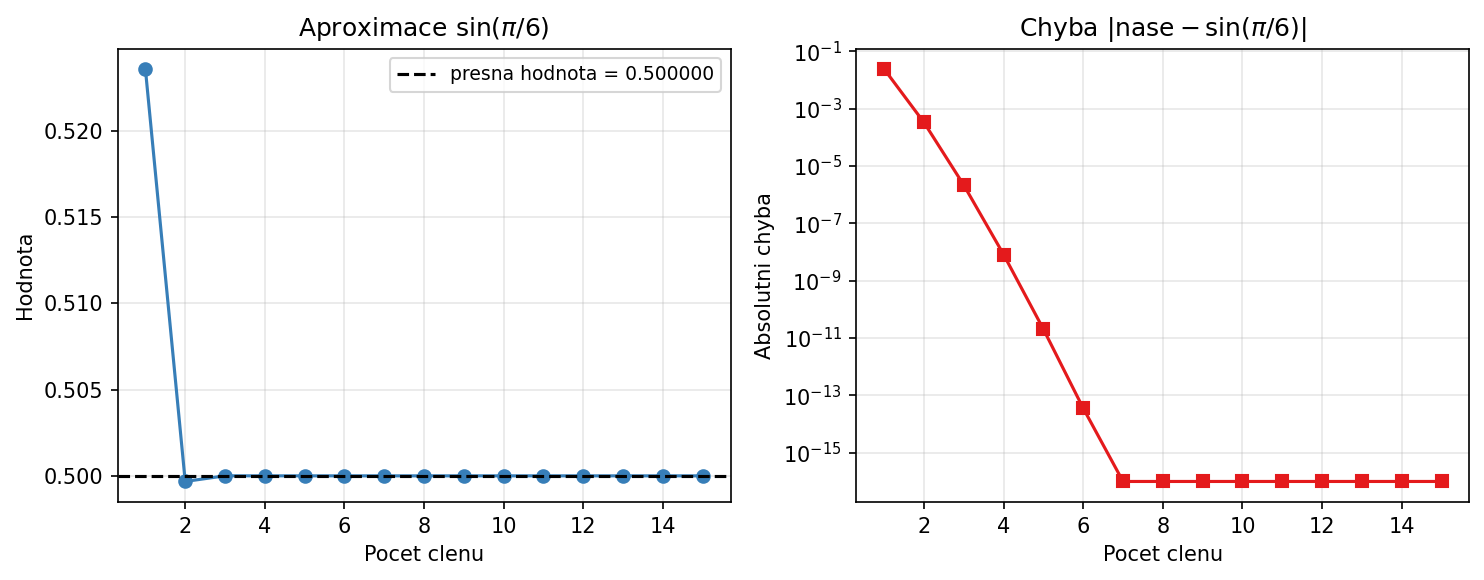
\includegraphics[width=\textwidth]{../python/output/sin_konvergence.png}
    \end{columns}

\end{frame}

% ----------------------------------------------------------
% SNÍMEK 13: Co se děje v praxi (range reduction, Čebyšev)
% ----------------------------------------------------------
\begin{frame}{Co se děje v~praxi}

    \begin{block}{Redukce oboru (\emph{range reduction})}
        Před výpočtem: přivedeme $x$ do intervalu
        $[0, \pi/2]$ pomocí $\sin(x + 2\pi) = \sin(x)$.\\
        Taylorova řada je pak přesná už při malém počtu členů.
    \end{block}

    \pause

    \begin{exampleblock}{Proč Čebyšev, ne Taylor?}
        Taylorův polynom stupně $n$ je přesný v~$x = 0$,
        ale na okraji intervalu dělá velké chyby.\\
        Čebyševův polynom rozloží chybu rovnoměrně
        na celém intervalu.
    \end{exampleblock}

    \pause

    \begin{alertblock}{CORDIC}
        Vyhýbá se násobení úplně.
        Používá se v~obvodech bez FPU
        (GPS, mikrokontroléry, FPGA).
    \end{alertblock}

\end{frame}

% ----------------------------------------------------------
% SNÍMEK 14: Literatura
% ----------------------------------------------------------
\begin{frame}[allowframebreaks]{Literatura}
    \printbibliography[heading=none]
\end{frame}

% ----------------------------------------------------------
% SNÍMEK 15: Shrnutí + zadání
% ----------------------------------------------------------
\begin{frame}{Shrnutí + domácí úloha}

    \begin{block}{Co jsme se naučili}
        \begin{itemize}
            \item Taylorova řada přibližuje funkci polynomem
            \item $\sin$ a $\cos$: lichými / sudými mocninami s~faktoriálem
            \item Odmocnina: Newtonova iterace (kvadratická konvergence)
            \item Kalkulačka: redukce oboru + Čebyšev / CORDIC
        \end{itemize}
    \end{block}

    \pause
    \begin{exampleblock}{Domácí úloha (viz zadání)}
        Implementujte \texttt{sin\_taylor(x, n)},
        \texttt{cos\_taylor(x, n)}, \texttt{sqrt\_newton(a, n)}
        v~čistém Pythonu.\\
        Porovnejte s~\texttt{math.sin} / \texttt{math.sqrt}
        pro alespoň 3 hodnoty.
    \end{exampleblock}

    \bigskip
    \centering
    \textbf{Děkuji za pozornost!}

\end{frame}

\end{document}
